\section*{Teoretický úvod}
		\subsection*{Bipolární tranzistor}
			\indent\indent
			Bipolární tranzistor je elektrotechnická součástka, oběvená 16. prosince 1947 v Bellových laboratořích týmem ve složení William Shockley, John Bardeen a Walter Brattain. Bipolární tranzistory mají tři elektrody: E - emitor, B - báze, C - kolektor. Bipolární tranzistory se dají rozdělit na tranzistory typu NPN a PNP. Jeden z nejdůležitějších parametrů tranzistoru je proudový zesilovací činitěl.
			
		\begin{equation}
  		\beta = \dfrac{\Delta I_C}{\Delta I_B}
  	\end{equation}
		
		\hspace*{2cm}kde:\newline    
  	\hspace*{4cm}$\beta$ \dotfill proudový zesilovací činitel\hspace*{4cm}\newline
  	\hspace*{4cm}$I_C$ \dotfill proud tekoucí kolektorem\hspace*{4cm}\newline
  	\hspace*{4cm}$I_B$ \dotfill proud tekoucí bází\hspace*{4cm}\newline
  				
			
			\begin{figure}[H]
        \centering
        \begin{subfigure}[b]{0.23\textwidth}
		      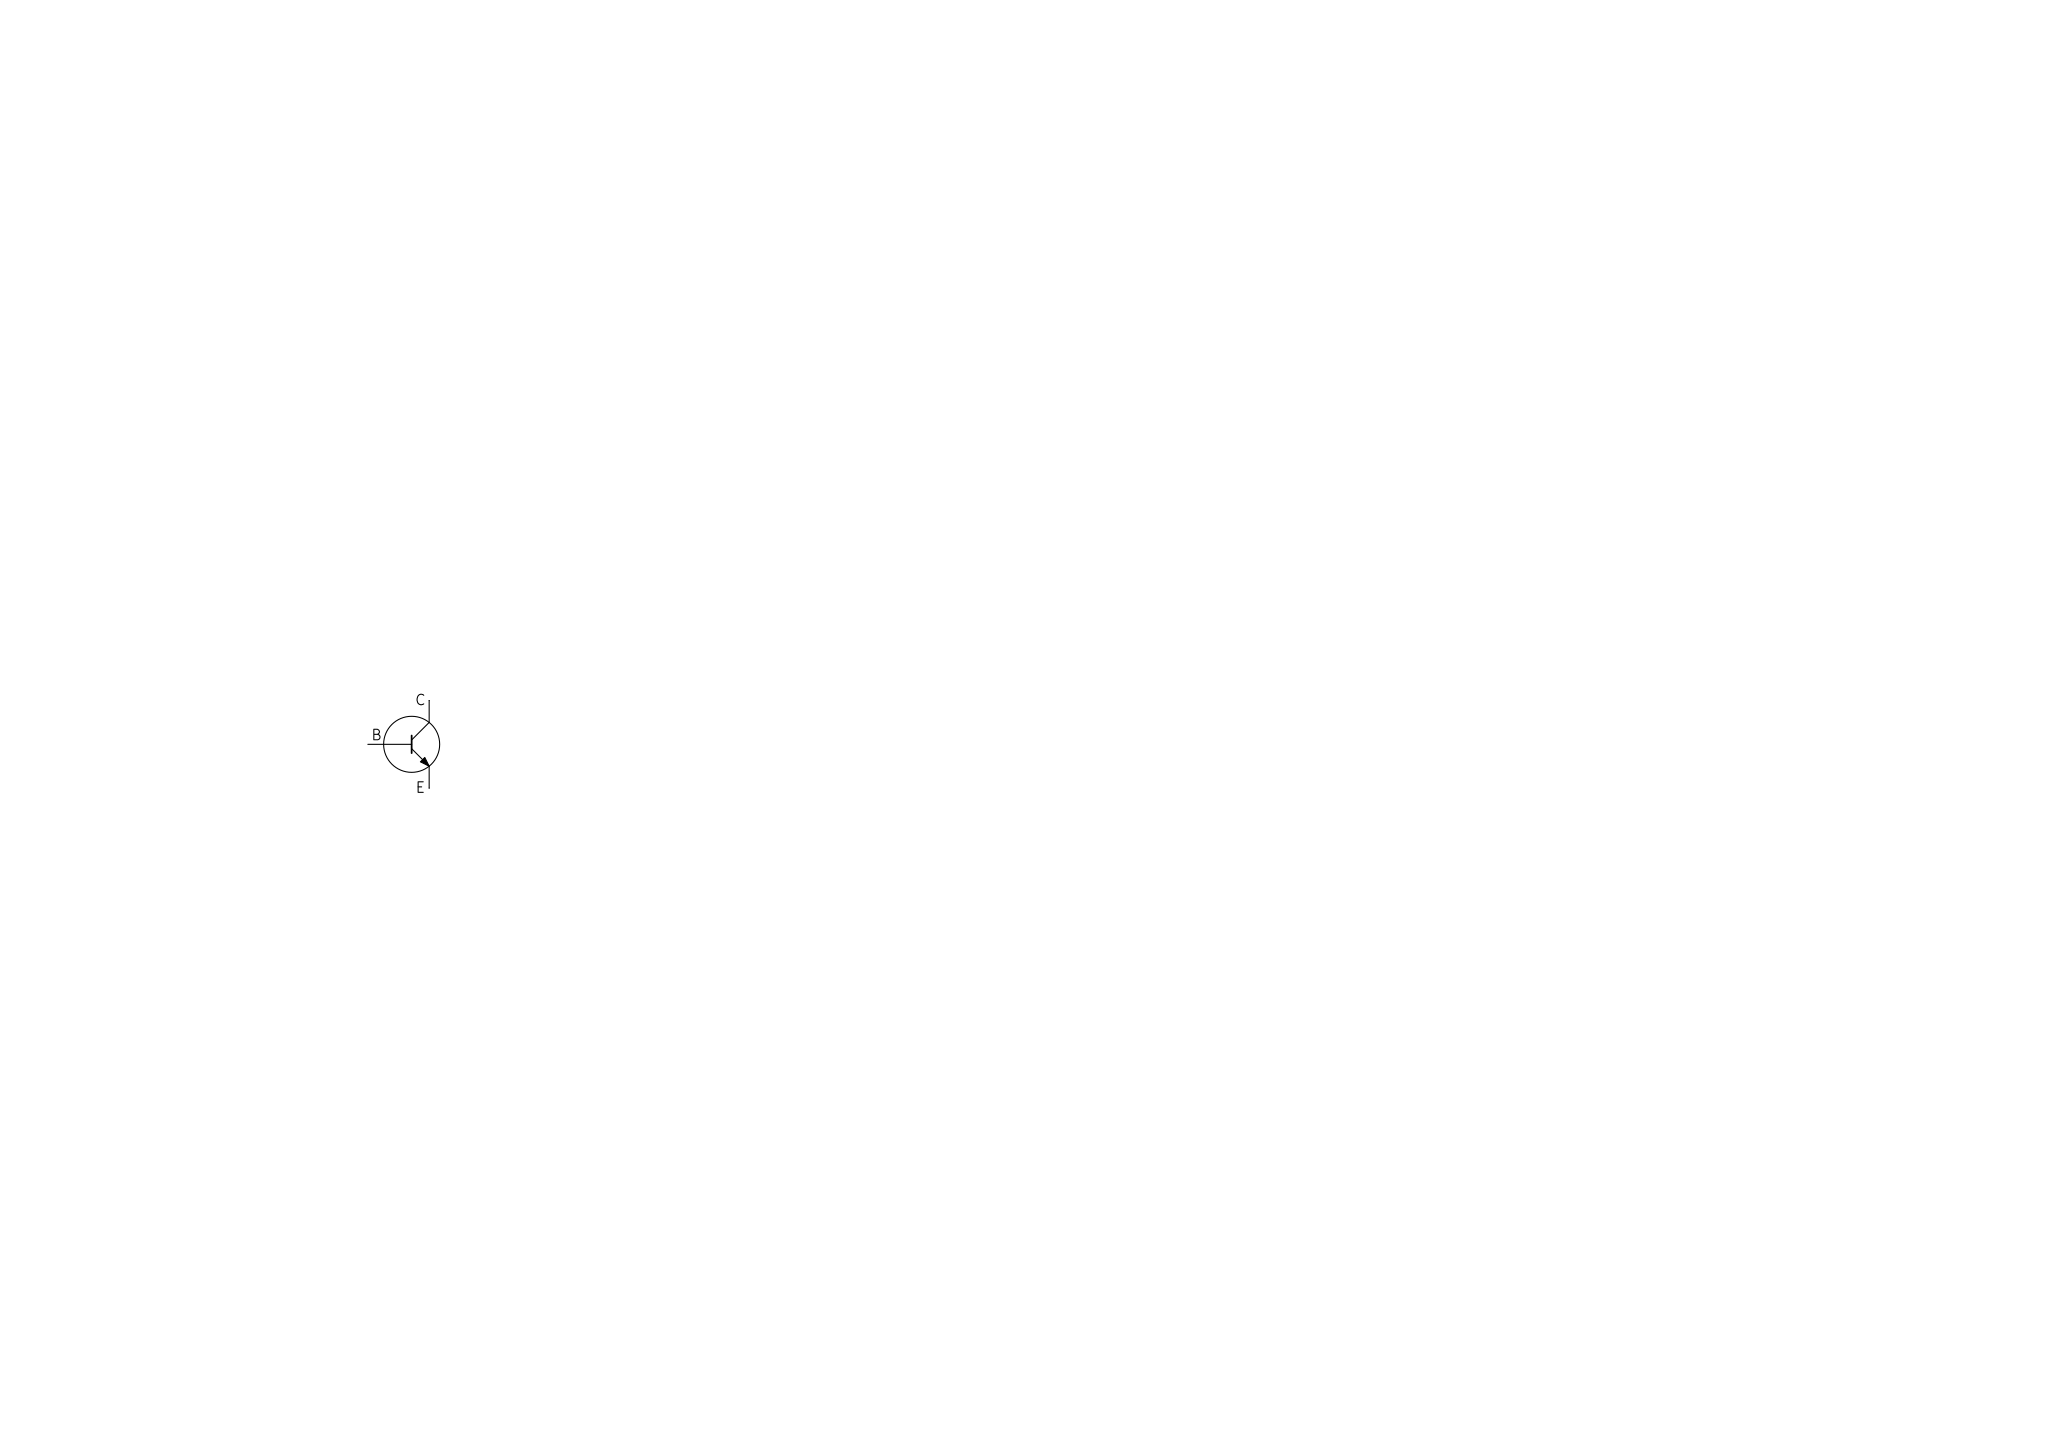
\includegraphics[width=22mm]{../img/NPN.pdf}
		      \caption{NPN značka}
		      %\label{fig:gull}
        \end{subfigure}%
        ~ %add desired spacing between images, e. g. ~, \quad, \qquad, \hfill etc.
          %(or a blank line to force the subfigure onto a new line)
        \begin{subfigure}[b]{0.23\textwidth}
          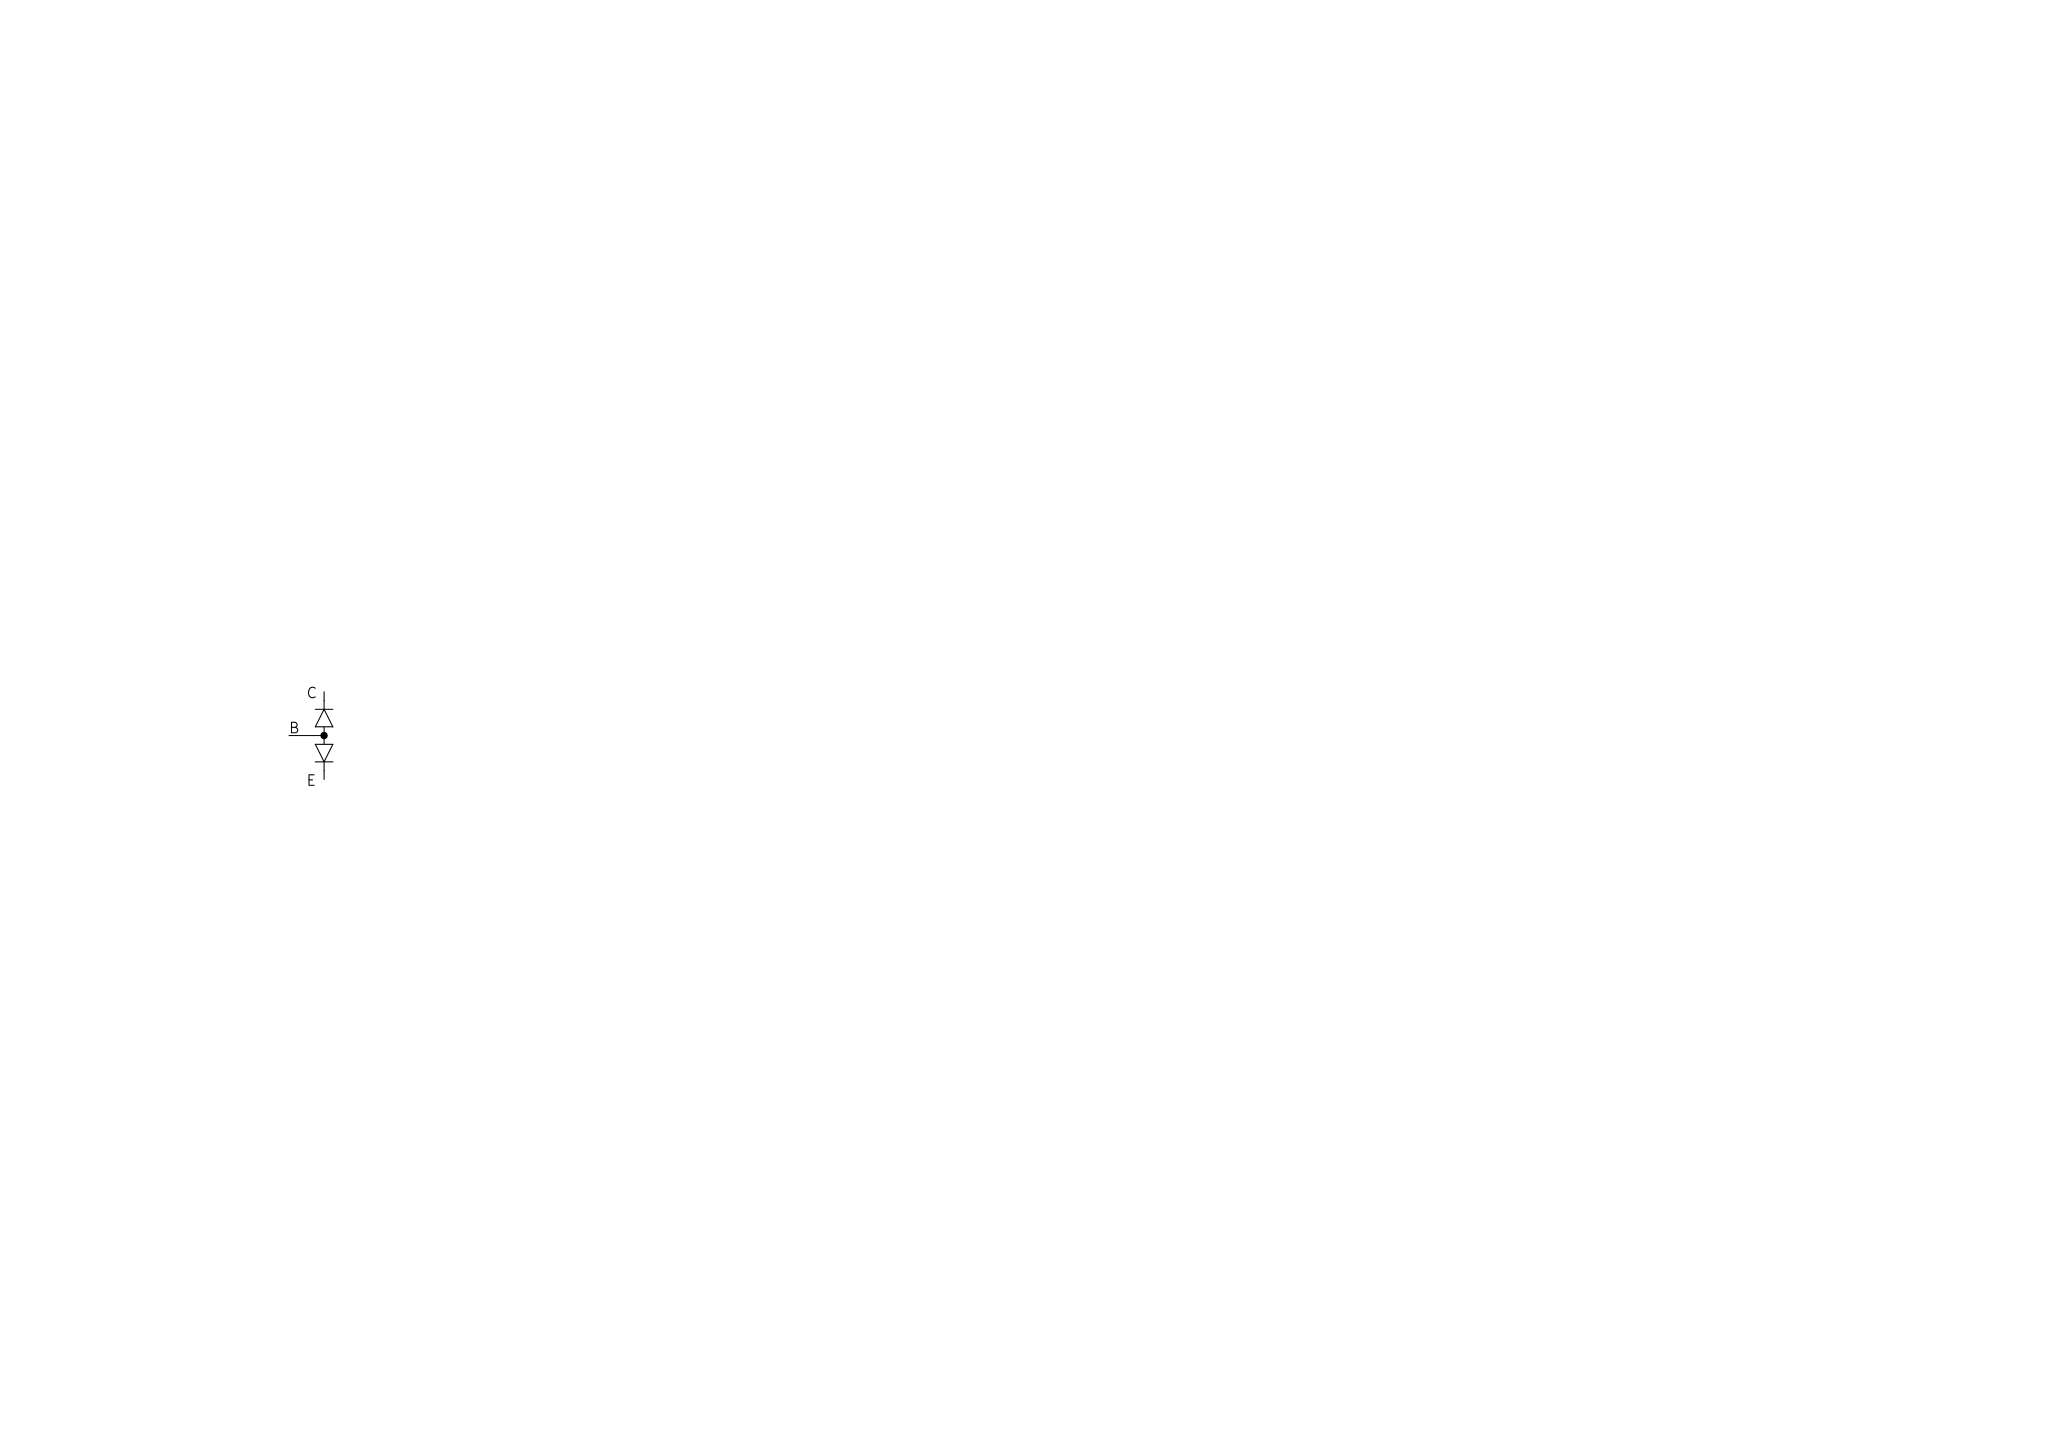
\includegraphics[width=13mm]{../img/NPN_D.pdf}
          \caption{NPN náhradní schéma}
          %\label{fig:tiger}
        \end{subfigure}
        ~ %add desired spacing between images, e. g. ~, \quad, \qquad, \hfill etc.
          %(or a blank line to force the subfigure onto a new line)
        \begin{subfigure}[b]{0.23\textwidth}
          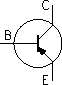
\includegraphics[width=22mm]{../img/PNP.pdf}
          \caption{PNP značka}
          %\label{fig:mouse}
        \end{subfigure}
         ~ %add desired spacing between images, e. g. ~, \quad, \qquad, \hfill etc.
          %(or a blank line to force the subfigure onto a new line)
        \begin{subfigure}[b]{0.23\textwidth}
          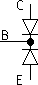
\includegraphics[width=13mm]{../img/PNP_D.pdf}
          \caption{PNP náhradní schéma}
          %\label{fig:mouse}
        \end{subfigure}
        
        \caption{schématické značky a náhradní zapojení bipolárních tranzistorů}
        \label{fig:tranzistory}
        
\end{figure}
			
			
		\subsection*{Zesilovač}
			\indent\indent
			Zesilovač je zařízení, které zesiluje vstupní signál. V této úloze je realizován pomocí tranzistoru KFY34 (NPN) v zapojení se společným emitorem. Toto zpojení otáčí fázi o $\pi~rad$. Hlavní parametr thoto zesilovače je napěťové zesílení.
			
			\begin{equation}
  			A_u = \dfrac{U_{OUT}}{U_{IN}}
			\end{equation}
	
			\hspace*{2cm}kde:\newline    
			\hspace*{4cm}$A_u$ \dotfill napěťové zesílení\hspace*{4cm}\newline
			\hspace*{4cm}$U_{IN}$ \dotfill vstupí napětí\hspace*{4cm}\newline
			\hspace*{4cm}$U_{OUT}$ \dotfill výstupní napětí\hspace*{4cm}\newline
  
  


